%!TEX root = ../main.tex
\documentclass[../main]{subfiles}
\ifSubfilesClassLoaded{
    \addbibresource{../Biblio/biblio.bib}
    \dominitoc
    \tableofcontentsfile
    \pagenumbering{arabic}
    \setcounter{page}{1}
    \setcounter{chapter}{2}
}{}

\begin{document}
\chapter{Méthodes de représentation et d'analyse de l'architecture CxSOM}\label{chap:repr}
\graphicspath{{04-Representation/figures},{./figures}}
\minitoc

\section{Introduction}

Nous avons proposé l'algorithme CxSOM, permettant de construire des architectures non-hiérarchiques de cartes auto-organisatrices.
Chaque carte de l'architecture a à la fois pour but d'extraire une représentation de ses entrées externes, tout en prenant comme entrée secondaire les positions des \emph{Best Matching Unit} d'autres cartes afin de prendre en compte les activités relatives aux différentes modalités dans le calcul de son BMU. 
Dans cette thèse, nous étudions les propriétés de l'architecture CxSOM dans un cadre particulier de mémoire associative.
L'objectif pour une architecture de cartes est d'apprendre une représentation des relations existant entre des entrées de différentes modalités, tout en apprenant une représentation au sein de chaque carte d'un espace d'entrée.
La compréhension du comportement de structures avec un faible nombre de cartes posera des bases pour la construction d'architectures plus grandes. Ce système de cartes est un système complexe, même dans une architecture de quelques cartes. Chaque carte possède 500 unités~; son état, représenté par son BMU, peut alors prendre 500 valeurs et l'état d'une carte dépend des cartes voisines.

L'objectif de cette thèse est d'observer comment l'organisation qui émerge d'une structure de cartes traduit un apprentissage associatif sur les entrées multimodales. Pour analyser l'organisation de ces cartes, nous aurons besoin de d'introduire de nouvelles représentations par rapport à celles utilisées dans les SOM classiques. 
Ce chapitre présente la méthode expérimentale et les représentations que nous utiliserons dans toutes les expériences présentées par la suite dans ce manuscrit.
Ces représentations ont pour but de qualifier la qualité de l'apprentissage, et surtout de mettre en lumière les propriétés et l'organisation des cartes émergeant de l'algorithme d'apprentissage.
La création de méthodes de représentation adaptées au modèle CxSOM sur une architecture élémentaire de peu de cartes nous permet de poser les bases pour l'étude de plus grandes architectures pour une suite à long terme des travaux.

\subsection{Présentation d'une expérience multimodale minimale illustrant les représentations}

La méthode expérimentale sera illustrée au long de ce chapitre sur un exemple d'une architecture de deux cartes, comme présenté au chapitre~\ref{chap:modele}.
L'architecture est illustrée à droite en figure~\ref{fig:exp}~: elle est composée de deux cartes en une dimension. Chaque carte prend une entrée externe, correspondant à $\inpx\m{1}=x$ et $\inpx\m{2}=y$, l'abscisse et l'ordonnée de points 2D sur un cercle. 
Ces deux modalités sont dépendantes~: pour une même valeur de $x$, deux valeurs sont possibles pour $y$, et symétriquement. Ce modèle d'entrée est représenté sur le schéma de gauche, figure~\ref{fig:exp}.
Nous normaliserons toutes les entrées sur $[0,1]$. Les entrées sont donc sur un cercle de centre $x_c,y_c = 0.5,0.5$ et de rayon $0.5$.

Chaque carte est une carte 1D de 500 n\oe{}uds, indexés par une valeur $p\m{i} \in [0,1]$.
La carte $M\m{1}$ prend en entrée contextuelle la position du BMU $\bmu\m{2}$ de $M\m{2}$, et inversement~; chaque carte possède donc une couche de poids externes et une couche de poids contextuels. Les rayons de voisinage choisis sont $h_e = 0.2$ et $h_c = 0.02$.
Afin de comprendre les tracés que nous présenterons, nous utiliserons deux autres cartes de Kohonen 1D classiques en tant que témoin.
Ces cartes prennent les mêmes valeurs d'entrées $\inpx\m{1}$ et $\inpx\m{2}$ que les cartes de l'architecture, mais ne sont pas connectées entre elles. 
Les paramètres de ces cartes sont les mêmes que les cartes de l'architecture~: chaque carte 1D compte 500 n\oe{}uds, le rayon de voisinage est constant $h_e = 0.2$. Ces cartes n'ont pas de poids contextuels.


\begin{figure}
\begin{minipage}{0.4\textwidth}
\centering
\includegraphics[width=0.8\textwidth]{2som_inp_noinformation}
\end{minipage}
\begin{minipage}{0.6\textwidth}
\includegraphics[width=\textwidth]{2som_archi}
\end{minipage}
\caption{A gauche, disposition des entrées dans l'exemple illustratif, sous forme de cercle. A droite, l'architecture de deux cartes en une dimension utilisée sur ces entrées dans ce chapitre pour illustrer les méthodes de représentation.\label{fig:exp}}
\end{figure}

\subsection{Représentations et indicateurs classiques des cartes de Kohonen}

Les cartes de Kohonen sont particulièrement associées à une facilité de représentation et de visualisation. Leur nombre réduit de prototypes et leur aspect topologique permet d'en tracer une représentation visuelle interprétable.
La manière la plus couramment utilisée de représenter une carte de Kohonen est de représenter les poids finaux de ses prototypes. 
Deux représentations sont souvent privilégiées~:
\begin{itemize}
\item Les prototypes de chaque n\oe{}ud sont tracés à leur emplacement $p$ sur la carte. 
C'est le cas sur l'exemple de gauche en figure~\ref{fig:representation} dans lequel les poids des prototypes, qui sont des imagettes 16x16, sont affichés en chaque point de la carte en deux dimensions.
\item Lorsque les données traitées sont des points deux ou trois dimensions, les poids des prototypes peuvent être directement tracés dans l'espace des entrées $\mathbb{R}^2$ ou $\mathbb{R}^3$. Les poids sont reliés en fonction des positions des n\oe{}uds dans la carte, montrant ainsi la déformation de la carte dans l'espace d'entrée, c'est le cas sur l'exemple de droite en figure~\ref{fig:representation} pour une grille en deux dimensions ayant appris sur des entrées en deux dimensions (en bleu).
\end{itemize}

Nous utiliserons des représentations adaptées au cas d'une architecture à plusieurs cartes à partir de ces deux modes de représentation.

\begin{figure}
\begin{minipage}{0.5\textwidth}
\centering
\includegraphics[width=0.5\textwidth]{digits.jpg}
\end{minipage}
\begin{minipage}{0.5\textwidth}
\centering
\includegraphics[width=0.5\textwidth]{points2.png}
\end{minipage}
\caption[Représentations classiques des poids d'une carte de Kohonen]{\label{fig:representation} Représentations possibles des poids d'une carte de Kohonen classique, dans le cas d'entrées sous forme d'imagettes ou de points en deux dimensions.\protect\footnote{Images tirées du \protect\href{polycopié d'apprentissage automatique}{https://frezza.pages.centralesupelec.fr/teachml2/Poly/Poly-ML-SDImetz.pdf} de CentraleSupelec Metz}}
\end{figure}
%\footnote{Images tirées du polycopié d'apprentissage automatique de CentraleSupelec Metz, 
%\url{https://frezza.pages.centralesupelec.fr/teachml2/Poly/Poly-ML-SDImetz.pdf}}
\subsection{Limites des représentations classiques dans le cas d'une architecture CxSOM}

Nous pouvons d'abord utiliser les représentations classiques mentionnées ci-dessus pour tracer les différentes couches de poids de chacun des cartes d'une architecture CxSOM à la fin de l'apprentissage.
La fin de l'apprentissage est définie comme le moment où les poids ont convergé vers une organisation restant stable au cours des itérations $t$.
La figure~\ref{fig:weights} présente le tracé des poids externes et contextuels des deux cartes de l'exemple selon leur position sur la carte, soit le pendant en une dimension de l'exemple de gauche en figure~\ref{fig:representation}.
La courbe orange correspond aux valeurs des poids externes de chaque carte.
Ce tracé permet d'observer que les poids externes couvrent l'intervalle $[0,1]$, et sont organisés de façon monotone, ce qui est l'organisation habituelle d'une carte classique se dépliant entre 0~et~1.
Les poids contextuels sont tracés en bleu. Ils ne présentent pas cette organisation monotone, mais font apparaître une organisation spatiale~: deux prototypes proches ont des poids proches. 
Le tracé des deux couches de poids nous informe donc sur le caractère ordonné de l'organisation de chacune de couches de poids. 

Notons que nous ne pouvons pas en tirer plus de conclusion~: la représentation des poids de la figure~\ref{fig:weights} ne différencie pas les n\oe{}uds qui seront effectivement BMUs, des n\oe{}uds dits \emph{morts}.
Ces n\oe{}uds morts ont bien un poids, mais ne seront jamais BMUs.
Dans une carte de Kohonen classique, les n\oe{}uds morts correspondent à des zones de transitions, liant deux zones denses de l'espace d'entrée séparées par une zone sans points.
Par ailleurs, cette représentation concerne une seule carte. Nous ne pourrons pas tirer de conclusion sur l'influence des connexions entre cartes à partir de cette seule représentation.

Au regard des insuffisances des représentations classiques, déjà révélées sur un cas très simple de deux cartes mono-dimensionnelles, nous constatons qu'il est nécessaire de trouver un moyen de représenter l'architecture comme un tout. Nous devons ainsi définir des représentations qui montrent comment l'architecture de cartes est capable d'apprendre les relations entre les entrées multimodales.

\begin{figure}
\centering
\includegraphics[width=0.9\textwidth]{weights_cercle1.pdf}

\caption{Représentation des valeurs des poids d'une carte au sein de CxSOM après apprentissage en fonction de leur position dans la carte. La seule représentation de ces poids ne suffit pas à savoir comment la carte se comporte.\label{fig:weights}}
\end{figure}

Suite aux limites montrées par les méthodes de représentation classiques utilisées dans le domaine des SOMs, ce chapitre propose plusieurs façons de représenter une carte au sein d'une architecture.
Nous présenterons en premier lieu une méthode expérimentale pour décrire les cartes et les entrées multimodales associées ainsi que la méthode expérimentale que nous utiliserons pour toutes les expériences présentées dans cette thèse. 
\'A partir de cette méthode, nous proposerons plusieurs représentations enrichies par rapport aux méthodes de représentation classiques, permettant de comprendre et représenter ce que calcule une architecture CxSOM sur les données d'entrées. Ces représentations seront illustrées sur l'exemple minimal de deux cartes pour faciliter la compréhension des comportements. Nous comparerons dans ce chapitre le comportement d'une architecture de deux cartes à celui de cartes classiques afin d'avoir une première idée des dynamiques d'apprentissage occurant dans CxSOM.
Nous utiliserons ensuite les méthodes de représentation dans les chapitres suivants pour analyser le comportement des cartes.

\section{Formalisation statistique des entrées et sorties des cartes}

Nous introduisons dans cette section un formalisme traitant les éléments des cartes et les entrées en tant que variables aléatoires. 
Ce formalisme possède à la fois l'avantage de clarifier les représentations et de permettre le développement d'indicateurs statistiques sur l'apprentissage effectué par les cartes.

\subsection{Formalisation des entrées}

Plaçons-nous dans le cas général d'une architecture de $n$ cartes pour formaliser davantage.
Nous considérons des entrées multimodales tirées d'un ensemble d'espaces d'entrée $\mathcal{D}\m{1},\cdots,\mathcal{D}\m{D}$. Chaque espace $\mathcal{D}\m{i}$ est une modalité de l'espace multimodal, avec $D$ le nombre de modalités considérées. Notons que comme une carte peut ne pas prendre d'entrée externe, $D \neq n$.
Les observations multimodales que l'on cherche à apprendre par l'architecture de cartes sont notées $(\inpx\m{i} \in \mathcal{D}\m{i}, i = 1 \cdots D)$.

Nous modélisons ces entrées $\inpx\m{i}$ comme des \emph{variables aléatoires} tirées selon une distribution $P\m{i}$ sur leur espace $\mathcal{D}\m{i}$.
$\mathbf{\inpx} = (\inpx\m{1}, \cdots, \inpx\m{n}) \in \mathcal{D}\m{1} \times \cdots \times \mathcal{D}\m{n}$ est la variable aléatoire jointe. 
Lors de chaque itération d'apprentissage, un vecteur $\mathbf{\inpx} = (\inpx\m{1}_t, \cdots , \inpx\m{n}_t)$ est présenté à l'architecture~: il s'agit d'une réalisation de la variable jointe $\mathbf{\inpx}$. 

En pratique, ces variables sont des observations, issues par exemple de capteurs d'un robot. Ces observations sont issues d'un environnement général et sont donc liées par des relations au sein de ce modèle d'environnement~: les variables $\inpx\m{i}$ ne sont pas des variables indépendantes.
Nous introduisons la notion de \emph{modèle d'entrées} se rapportant à cette dépendance entre variables.
Le modèle d'entrée fait référence au modèle d'environnement permettant de générer les entrées multimodales fournies en entrée de l'architecture. Dans l'exemple d'illustration, les modalités sont les abscisses $\inpx\m{1} = x$ et les ordonnées $\inpx\m{2} = y$~; le modèle d'entrées est le cercle sur lesquels sont situés les points, modélisé par exemple par l'équation $(x - 0.5)^2 + (y - 0.5)^2 = 0.5^2$.

\subsection{Formalisation du modèle d'entrée par une variable cachée}

Un modèle d'environnement peut être paramétrisé par une variable multidimensionnelle $U$. 
Les modalités sont alors définies comme des fonctions de cette variable~:
$\inpx\m{i} = f\m{i}(U)$
$U$ est une nouvelle variable aléatoire, décrivant l'ensemble des paramètres du modèle.

Pour que la variable $U$ conserve toute l'information sur le modèle d'entrées, la fonction $(f\m{1}, \cdots, f\m{n})$ : $(\inpx\m{1}, \cdots \inpx\m{n})\rightarrow U$ doit être une bijection. Toute valeur d'entrées jointes correspond à un seul $U$, toute valeur de $U$ renvoie à une seule valeur d'entrées jointes. 
On peut considérer cette paramétrisation comme un cas particulier de réduction de dimension du modèle, dans lequel la variable $U$, de dimension plus faible que $\mathbf{X}$, réduit la dimension des entrées sans perte d'information.

La variable $U$ s'interprète par l'existence d'une variété de dimension inférieure ou égale à la dimension des entrées, sur lesquelles les entrées multimodales se trouvent.
Des travaux font l'hypothèse que des variables en grande dimension, telles que des images, sont positionnées en pratique sur des variétés de dimension plus faible \cite{Pless2009ASO}, dont un exemple est donné en figure~\ref{fig:U}.
L'utilisation de variables d'entrées multimodales placées sur une variété inférieure, en faible dimension dans notre étude, est ainsi un cadre d'expériences généralisable.
Par ailleurs, les méthodes existantes de réduction de dimension non-linéaire permettent d'extraire des structures dans des données réelles. 
Ainsi, bien que nos travaux se concentrent sur des données en faible dimension, la représentation paramétrique est généralisable à des données de plus grande dimension ainsi qu'à des jeux de données réelles. 
On peut voir la variable $U$ comme un cas particulier de réduction de dimension sans perte d'information~; cependant, les représentations proposées seront également adaptables à une variable $U$ obtenue par une réduction de dimension avec perte d'information (par exemple par une PCA). 

\begin{figure}
    \begin{minipage}{0.4\textwidth}
    \centering
    \includegraphics[width=0.8\textwidth]{pless-000.png}
    \end{minipage}
    \begin{minipage}{0.6\textwidth}
    \centering
    \includegraphics[width=0.9\textwidth]{2som_inp.pdf}
    \end{minipage}
    \caption{
        \'A gauche, ensemble d'images représentant une statuette sous différents angles de vue. Toutes les images, de grande dimension, sont situées sur une variété 3D sous-jacente représentant la rotation de la caméra.(Source~:~\cite{Pless2009ASO}).
       La figure de droite présente le pendant en deux dimensions présentant également cette propriété. Les modalités 1D $\inpx\m{1}$ et $\inpx\m{2}$ sont placées sur un cercle qui est une variété en une dimension. Ce modèle est paramétrisé par la variable $U$. Nous utilisons ce modèle d'entrée comme exemple dans ce chapitre.
       \label{fig:U}}
\end{figure}

Les points de l'espace d'entrée pris en exemple, représentés à droite en figure~\ref{fig:U} sont paramétrisés par leur angle sur le cercle $U$ qui est une variable 1D représentant le modèle d'entrées~:
\begin{equation}
 \begin{cases}
     \inpx\m{1}= x_c + r  \cos(2\pi U)\\
     \inpx\m{2} = y_c + r \sin(2 \pi U)
    \end{cases}\,.
\end{equation}

$U$ est aussi une variable aléatoire. Sa valeur n'est pas fournie à l'architecture de cartes lors de l'apprentissage, il s'agit d'une variable latente.
Nous cherchons, par l'architecture de cartes, à apprendre les entrées et les relations entre entrées~: nous cherchons donc à extraire une structure dans le modèle latent. La relation entre $U$ et $\mathbf{X\m{i}}$ est bijective~; de ce fait, étudier comment l'architecture de cartes a appris $U$ est équivalent à étudier comment l'architecture a appris le modèle d'entrées.
Cet exemple est scalaire mais la représentation sous forme de variable cachée est générale à n'importe quel dimension et nombre d'entrées. 
En effet, toute configuration d'entrée multimodale dépend d'un environnement global. La variable $U$ correspond alors aux paramètres de cet environnement.

\subsection{Formalisation des éléments des cartes}

Afin d'étudier le comportement d'une carte à n'importe quel instant $t$ de l'apprentissage, nous effectuons des phases de \emph{test}, décrit en figure~\ref{fig:flowchart}.
Lors d'une phase de test, les poids des cartes ne sont pas mis à jour. Chaque entrée génère une recherche de BMU par relaxation, donc un ensemble d'élément de réponse de la carte aux entrées présentées. Ces éléments de réponse sont les activités externes et contextuelles, la position du BMU, le poids du BMU ou tout autre quantité observable à partir de l'état des cartes.
Les entrées utilisées lors du test sont un échantillon de la variable aléatoire $(\inpx\m{1}, \cdots, \inpx\m{n})$.
La distribution des entrées test est identique à la distribution des entrées d'apprentissage ayant servi au dépliement de la carte.

Nous avons représenté les entrées comme des variables aléatoires~; chaque élément de réponse des cartes d'une architecture sera également considéré comme une variable aléatoire.
Nous choisissons en particulier de nous intéresser aux positions des BMUs $\bmu\m{1}, \cdots, \bmu\m{n}$ et à leurs poids $\w\ext\m{1}(\bmu\m{1})$ et $\w\ext\m{2}(\bmu\m{2})$.
Comme les poids ne sont pas mis à jour entre chaque itération de test, toutes les valeurs obtenues lors d'une phase de test forment un échantillon de la variable aléatoire jointe suivante~:
$$(\underbrace{\inpx\m{1}, \cdots, \inpx\m{n}, U,}_{\text{Entrées}} \underbrace{\bmu\m{1}, \cdots, \bmu\m{n}, \w_e\m{1}(\bmu\m{1}), \cdots, \w_e\m{n}(\bmu\m{n})}_{\text{Eléments de réponse}})$$

Les composantes de cette variable jointe ne sont pas indépendantes et étudier l'apprentissage revient à étudier les dépendances se créant entre les composantes.
Les représentations présentées par la suite constituent les tracés des dépendances au sein d'un échantillon de test entre les composantes de la variable jointe définie ci-dessus.

Les variables d'entrées sont à valeurs continues et $\bmu$ à valeurs discrètes, correspondant aux 500 n\oe{}uds d'une carte. 
Nous pouvons cependant aussi considérer $\bmu$ comme une variable continue plutôt qu'une grandeur discrète. 
En effet, l'ensemble des positions du BMU correspondent à une discrétisation de l'espace continu $[0,1]$, et sont ordonnées. Le déplacement par relaxation n'est pas limité aux positions discrètes des BMUs.
Ce cadre statistique permettra aussi d'utiliser des outils et métriques issus de la théorie de l'information pour qualifier l'organisation des cartes au sein de l'architecture, ce que nous ferons dans le chapitre~\ref{chap:indicateur}

\begin{figure}
\centering
\includegraphics[width=0.85\textwidth]{tests_2maps.pdf}
\caption{Schéma décrivant une étape de test. Un test consiste à présenter successivement des réalisations de $\mathbf{X}$, notées $(\inpx\m{1}_t,\inpx\m{2}_t)$. Nous laissons le processus de relaxation stabiliser les BMUs. Quand la stabilité est atteinte, la valeur des positions de BMU $\bmu\m{1}_t$ et $\bmu\m{2}$ est obtenue. Les poids ne sont pas mis à jour entre chaque itération, ce qui permet de considérer une phase de test comme un échantillonnage de la variable aléatoire $(\inpx\m{1},\inpx\m{2}, U, \bmu\m{1}, \bmu\m{2}$) }
\label{fig:flowchart}
\end{figure}

\section{Représentations graphiques}

\`A partir des échantillons de test, nous proposons dans cette section les représentations graphiques que nous utiliserons pour évaluer expérimentalement les architectures de cartes.
Ces représentations sont toutes un tracé de dépendances entre certaines composantes de la variable $$(\inpx\m{1}, \cdots, \inpx\m{n}, U, \bmu\m{1}, \cdots, \bmu\m{n}, \w_e\m{1}(\bmu\m{1}), \cdots, \w_e\m{n}(\bmu\m{n}),U)$$ dont un échantillon est obtenu lors du test.

\subsection{Erreur de quantification d'une modalité dans chaque carte}

La première fonction d'une carte de Kohonen est de réaliser une tâche de quantification vectorielle sur son entrée externe. Au sein d'une architecture de cartes, nous nous attendons à ce que chaque carte extraie une représentation de la modalité qu'elle prend en entrée externe.
Afin de mesurer cette qualité de quantification vectorielle au sein d'une carte dans CxSOM, nous traçons le nuage de points correspondant au poids externe du BMU $\w_e(\bmu\m{i})$ en fonction de l'entrée externe présentée $\inpx\m{i}$. Une carte effectue une quantification vectorielle correcte si ce nuage de points est proche de la fonction identité.
Ces tracés sont réalisés en figure~\ref{fig:erreur} pour l'expérience exemple. Ces tracés s'approchent de l'identité, ce qui montrent la quantification des entrées est correctement réalisée.
On pourrait mesurer une erreur quadratique moyenne pour déterminer numériquement cette erreur de quantification mais la représentation en nuage de points est, à défaut d'être quantitative, plus qualitative. 
En effet, ici, on observe que le nuage montre une structure \og filamenteuse \fg{}. Nous reviendrons sur ce point par la suite, nous contentant de souligner ici que la représentation graphique exprime une propriété que la simple mesure d'erreur n'aurait pas mis en évidence.

Cette représentation nous informe ainsi sur la qualité de quantification dans une seule carte relativement à une seule modalité. Cette seule représentation est insuffisante à elle seule pour comprendre plus en détail le comportement d'une architecture de cartes~: il nous faut également définir des méthodes de représentation permettant d'évaluer comment la structure globale du modèle d'entrées est apprise par l'architecture dans son ensemble.

\begin{figure}
    \centering
    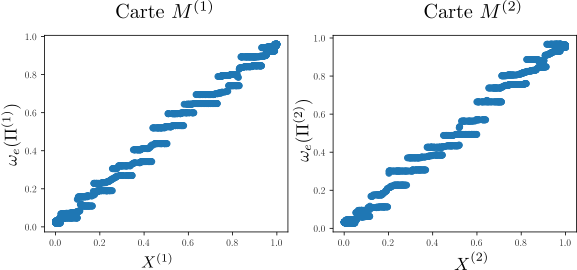
\includegraphics[width=0.7\textwidth]{w_x.pdf}
    \caption{Poids du BMU dans chaque carte en fonction de l'entrée présentée. On s'attend à des tracés proches de l'identité, montrant que le poids du BMU d'une carte est une bonne représentation de l'entrée. Ces tracés montrent que la quantification vectorielle est correctement réalisée, et que plusieurs BMUs correspondent à une même valeur d'entrée, d'où la structure filamenteuse. \label{fig:erreur}}
\end{figure}


\subsection{Représentation cartographique des valeurs d'entrées préférentielles des BMUs}

En biologie, les aires du cortex cérébral sont cartographiées en faisant varier le motif d'entrée dans son espace, et en indiquant pour chaque neurone la valeur d'entrée préférentielle à laquelle il réagit. Cela donne alors une représentation cartographique où des valeurs de l'espace d'entrée sont tracées par rapport à la position sur le substrat neuronal du neurone qui y réagit.
Par exemple, une carte corticale est tracée pour l'aire visuelle primaire du cortex cérébrale, l'aire v1, en figure~\ref{fig:v1_repr}.

Un échantillon test donne un ensemble de valeurs de variable jointe $(\inpx\m{1}, \cdots, \inpx\m{n}, \bmu\m{1},\cdots, \bmu\m{n})$. Dans la même idée que les cartes corticales, nous tracerons à partir de l'échantillon de test le nuage de points correspondant à la valeur de l'entrée $\inpx\m{i}$ d'une carte par rapport à la position du BMU $\bmu\m{i}$.

En figure~\ref{fig:inputs}, nous avons tracé cette représentation cartographique pour l'exemple à deux cartes. Le cas de la 1D permet de mettre en relation plusieurs éléments sur un même graphique.
Le tracé relatif à une des cartes $M\m{i}$ contient les éléments suivants~:
\begin{itemize}
    \item Les courbes des poids externes et contextuels de la carte $w_e$ et $w_c$ en fonction des positions $p$ dans la carte.
    \item Les entrées externes $\inpx\m{i}$ en fonction de la position de leur BMUs $\bmu\m{i}$. On s'attend à ce que ces points soient proches de la courbe de poids externe si la quantification vectorielle est bien réalisée
    \item Les entrées externes des autres cartes $\inpx\m{k}$ en fonction de $\bmu\m{i}$. Le tracé de ces entrées permet de faire apparaître les paires d'entrées présentées ensemble à l'architecture.
\end{itemize} 

Deux valeurs issues de l'échantillon de test sont mise en évidence en couleur rouge et bleue sur chaque graphique. Un point de même couleur correspond à un même élément test dans chaque graphique. Ces deux points partagent la même abscisse, c'est-à-dire que l'entrée $\inpx\m{1}$ est la même pour ces deux éléments. Par contre, leur ordonnée est différente~: $M\m{2}$ a reçu donc une entrée $\inpx\m{2}$ différente.

Ce tracé nous permet d'abord d'observer que les points $(\bmu\m{1},\inpx\m{1})$ sont proches de la courbe de poids externes~: le poids d'un BMU est proche de l'entrée qui a été présenté et est donc une bonne approximation de cette entrée. Cela permet de conclure que la quantification vectorielle est bien réalisée dans cette carte sur les entrées externes, comme le montrait déjà la figure~\ref{fig:erreur}.

Tracer les échantillons de test permet ensuite d'observer la répartition des BMUs sur la carte. Les poids externes de la carte dans CxSOM (c) et de la carte indépendantes (b) sont organisés de façon monotone sur l'intervalle d'entrées $[0,1]$.
La représentation cartographique fait apparaître des zones mortes, sans BMUs. 
Nous observons que la carte au sein de CxSOM est découpée en plusieurs zones dans lesquelle les unités sont BMUs, séparées par des petites zones mortes. Ce tracé permet donc d'identifier un comportement qui est spécifique à une architecture de cartes CxSOM, par rapport à une carte classique. Nous reviendrons sur ce comportement dans les chapitres suivants.

Enfin, les nuages de points $(\bmu\m{1},\inpx\m{1})$ et $(\bmu\m{1},\inpx\m{2})$ nous permettent d'observer quelles valeurs d'entrées sont encodées à quelles positions dans la carte.
Nous observons grâce à ces tracés que sur la carte $M\m{1}$, le choix du BMU permet d'ordonner les entrées selon la valeur de $\inpx\m{1}$ mais également selon la valeur de $\inpx\m{2}$. 
Les points bleus et rouges apparaissent à deux positions différentes sur la figure~: leurs deux BMUs sont différents, bien qu'ils aient la même valeur de $\inpx\m{1}$. Dans la carte simple, ces deux entrées ont le même BMU.
Le comportement est similaire sur la carte $M\m{2}$. Le type de tracé montre ainsi une différence de répartition des BMUs qui n'est pas seulement liée aux poids externes et n'est pas mise en évidence par le tracé des seuls poids.
Nous étudierons dans les chapitres suivants comment ce comportement se généralise pour différentes architectures et distributions d'entrées grâce à la représentation cartographique présenté ici.

\begin{figure}
    \centering
    \includegraphics[width=0.7\textwidth]{v1.jpg}
    \caption{Carte corticale de l'aire cérébrale visuelle V1. Pour tracer cette représentation, un ensemble de traits de différentes orientations sont présentés en stimuli visuels au sujet, indiqués en bas de l'image. Le neurone réagissant à une entrée d'orientation particulière est coloré sur la carte de la couleur correspondante à l'entrée. Cette méthode permet de tracer des \emph{cartes corticales} d'une aire cérébrale \cite{Bosking1997OrientationSA}. \label{fig:v1_repr}}
\end{figure}

\begin{figure}
\begin{minipage}{0.27\textwidth}
\includegraphics[width=\textwidth]{2som_inp_noU.pdf}
\end{minipage}
\begin{minipage}{0.34\textwidth}
\includegraphics[width=\textwidth]{weights_2som_unco.pdf}
\end{minipage}
\begin{minipage}{0.38\textwidth}
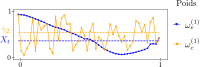
\includegraphics[width=\textwidth]{weights_2som.pdf}
\end{minipage}

\caption{Représentation des entrées $\inpx\m{1},\inpx\m{2}$ d'une architecture de deux cartes relativement au BMU de la carte $M\m{1}$ après apprentissage. Ces tracés mettent en valeur l'organisation des cartes qui sont différentes dans le cas ou les cartes apprennent indépendamment leurs entrées~(b) ou sont connectées~(c). Les entrées correspondantes sont en figure~(a). Les points bleu et rouge reportés sur les tracés correspondent au même échantillon de test.\label{fig:inputs}}
\end{figure}

\subsection{Représentation de la variable cachée selon les positions des BMUs}

La représentation cartographique permet de montrer que sur chaque carte $M\m{i}$, les BMUs sont organisées selon les valeurs de l'entrée externe $\inpx\m{i}$ mais aussi selon les valeurs d'entrées des autres cartes. Chaque carte s'organise ainsi en fonction du \emph{modèle d'entrée}, donc en fonction de $U$.
Afin de mettre en valeur ce comportement, nous pouvons tracer $U$ en fonction de la position $\bmu\m{i}$ du BMU de chaque carte, que nous représentons en~figure~\ref{fig:piu} sur le cas d'exemple.

Ce tracé fait apparaître $U$ comme une fonction de la position du BMU dans chaque carte, contrairement au cas où les cartes ne sont pas connectées. 
Cela traduit bien le fait que chaque carte a appris une représentation du modèle d'entrée et non seulement de la disposition des entrées externes.
Ce type de représentation permet de réduire la dimension des entrées à tracer et sera ainsi adaptée pour des architectures de plus de cartes et des entrées de dimensions supérieures.
Cette représentation fait clairement apparaître $U$ comme une fonction de $\bmu$ dans chaque carte. Ce comportement traduit dans cet exemple le fait que les cartes s'organisent en fonction de tout le modèle d'entrée, non seulement de leur entrée externe.

\begin{figure}
\centering
\includegraphics[width = \textwidth]{xu_yu_both.pdf}
\caption{Valeur de $U$ en fonction des valeurs du BMU $\bmu\m{i}$ dans chacune des cartes dans l'exemple d'illustration. Sur la première ligne, nous traçons la réponse de chaque carte à son entrée dans le cas ou les deux cartes ne sont pas connectées. Sur la deuxième ligne, nous traçons la réponse de chaque carte lorsqu'elles ont appris de façon jointe au sein de CxSOM.
$U$ apparaît alors comme une fonction de la position du BMU $\bmu\m{i}$ dans chaque carte, contrairement au cas où les cartes apprendraient indépendamment sur les mêmes entrées. Cette relation fonctionnelle est symbolisée par les pointillés sur les tracés du bas. Les mêmes échantillons rouge et bleu mis en évidence en figure~\ref{fig:inputs} sont reportés sur les tracés.}
\label{fig:piu}
\end{figure}

\subsection{Dépliement d'une carte dans l'espace d'entrée multimodal}

Une des représentations classiques des cartes de Kohonen est de tracer les poids de la carte dans l'espace de ses entrées, telle qu'en figure de droite en~\ref{fig:representation}. Cette représentation permet de faire apparaître un dépliement des poids d'une carte sur ses entrées.
De la même façon, nous voulons représenter comment chaque carte se déplie dans l'espace non seulement de ses entrées externes, mais dans l'espace multimodal, ce qui est possible à partir des échantillons de test.

Nous définissons une façon de représenter le dépliement d'une seule carte de CxSOM dans l'espace global des entrées. Dans l'exemple, il s'agit de représenter le dépliement de $M\m{1}$ selon $(\inpx\m{1},\inpx\m{2})$.
Au lieu de s'appuyer sur les poids des cartes comme en~\ref{fig:representation}, nous utilisons les valeurs de l'échantillon de test. Cette représentation est tracée en ~\ref{fig:distortion} pour l'exemple à deux cartes.
Nous traçons sur cette figure le nuage de poids correspondant au poids des BMUs selon leur position lors d'un test~: $\left( \w_e\m{1}(\bmu\m{1},\w_e\m{2}(\bmu\m{2}) \right)$. Nous relions ces points selon l'ordre de leurs positions dans la carte $M\m{1}$ pour tracer $M\m{1}$, de même pour $M\m{2}$. Nous obtenons ainsi une représentation des cartes $M\m{1}$ ou $M\m{2}$ dépliées dans l'espace global des entrées. 
Notons que les unités mortes ne peuvent pas être représentées sur la carte de cette façon. Nous ne représentons que les BMUs. 

Comme les poids externes représentent directement la valeur de l'entrée externe, on s'attend à ce que la forme du nuage de points corresponde à la structure globale des entrées.
Les tracés mettent en lumière les propriétés observées lors de la représentation cartographique des entrées, à savoir l'apparition de zones dans chaque carte. 
Les poids suivent la structure circulaire des entrées en découpant l'espace en zones et marquent les potions du cercle qui sont effectivement représentées par les poids.
Ce dépliement met en valeur la façon dont est parcouru l'espace dans chaque carte~: en fonction de $\inpx\m{1}$ dans la carte $M\m{1}$, et en fonction de $\inpx\m{2}$ dans la carte $M\m{2}$.
Cette représentation offre la possibilité  de visualiser comment une carte se déplie dans l'espace d'autres modalités. En particulier, nous pourrons visualiser le dépliement d'une carte de l'architecture qui ne prendrait pas d'entrée externe.

\begin{figure}
    \begin{minipage}{0.49\textwidth}
    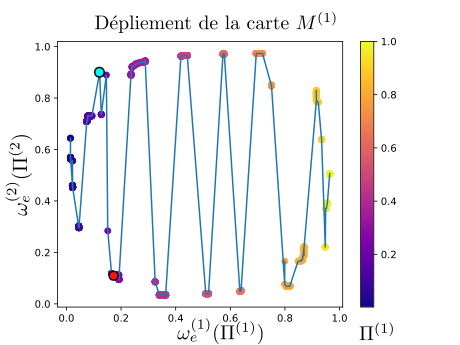
\includegraphics[width=\textwidth]{disto_cercle_M1.pdf}
    \end{minipage}
    \begin{minipage}{0.49\textwidth}
    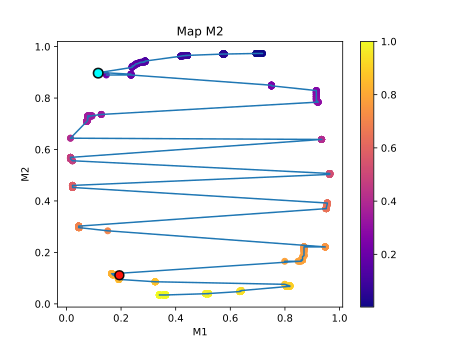
\includegraphics[width=\textwidth]{disto_cercle_M2.pdf}
    \end{minipage}
    \caption{Dépliement des cartes $M\m{1}$ et $M\m{2}$, reliés dans l'ordre de leurs positions selon $M\m{1}$ figure de gauche et $M\m{2}$ figure de droite. Le dépliement de chacune des cartes est alors représenté dans l'espace complet des entrées \label{fig:distortion}. L'indice du BMU est signalé par la carte de couleurs, différenciant ainsi les extrémités en 0 et 1 des cartes.}
    \end{figure}

\section{Conclusion}

Nous avons présenté dans ce chapitre une méthode expérimentale et des représentations pour l'analyse d'une architecture de cartes, que nous utiliserons dans les chapitres suivants.
Les représentations s'appuient sur des échantillons tests pouvant être réalisés tout au long de l'apprentissage.
Nous modélisons les entrées ainsi que les éléments des cartes comme des variables aléatoires et l'étape de test comme l'échantillonnage d'une variable jointe. 
La représentation des réponses aux tests permet de mieux comprendre les mécanismes des cartes, reposant sur un processus dynamique de recherche du BMU, que la simple observation de leurs poids.

Nous utiliserons donc quatre représentations des cartes dans la suite de cette thèse, toutes définies à partir d'un échantillon de test~:
\begin{itemize}
    \item Le tracé du poids du BMU en fonction de l'entrée externe permet d'évaluer la quantification vectorielle d'une carte.
    \item La représentation cartographique des entrées selon le BMU permet de faire apparaître quels positions encodent quelles valeurs d'entrées. Elle fait notamment apparaître des zones mortes dans la carte. Cette représentation met en lumière un comportement émergeant de l'exemple à deux cartes~: de façon auto-organisée, chaque carte ordonne ses BMUs selon le couple d'entrées $(\inpx\m{1},\inpx\m{2})$, et non seulement $\inpx\m{1}$.
    \item Le tracé de $U$ selon les positions des BMUs $\bmu\m{i}$ résume la représentation cartographique des entrées. Nous observons en particulier que l'apprentissage du modèle d'entrée se traduit par l'observation d'une relation fonctionnelle entre $U$ et $\bmu$ dans chaque carte.
    \item Enfin, nous proposons une représentation du dépliement de chaque carte dans l'espace de toutes les entrées en traçant les poids externes des BMUs de l'architecture, ordonnés selon les valeurs des positions dans une des cartes. Cette représentation apporte une vision globale de la façon dont une carte encode le modèle d'entrées.
\end{itemize}

Nous reviendrons au chapitre~\ref{chap:analyse} sur les conclusions que nous pouvons tirer de l'expérience illustrative du cercle et compléterons cette analyse sur d'autres dispositions d'entrées et architectures.
Même avec des représentations adaptées, l'analyse d'architectures comportant de nombreuses cartes ne peut pas simplement s'effectuer à l'aide de graphiques, qui deviendraient trop chargés. 
La comparaison d'un grand nombre d'expériences est également difficilement réalisable graphiquement.
Cette difficulté de représentation et le besoin de comparer des expériences soulève la nécessité de définir des valeurs indicatrices du fonctionnement de la carte, que nous proposerons au chapitre \ref{chap:indicateur}.
 
\ifSubfilesClassLoaded{
    \printbibliography
    %\externaldocument{../main.tex}   
}{}
\end{document}